 \documentclass[conference]{IEEEtran}

\IEEEoverridecommandlockouts
% Add the compsoc option for Computer Society conferences.
%
% If IEEEtran.cls has not been installed into the LaTeX system files,
% manually specify the path to it like:
% \documentclass[conference]{../sty/IEEEtran}


\usepackage{listings}
\usepackage{url}
\usepackage{graphicx}
\usepackage{numprint}
\usepackage{array,multirow}
\usepackage{multicol}
\usepackage{amssymb}
\usepackage{tikz}
\usepackage[autostyle]{csquotes}



\newtheorem{rem}{Remark}
\newtheorem{example}{Example}
% Some very useful LaTeX packages include:
% (uncomment the ones you want to load)


% *** MISC UTILITY PACKAGES ***
%
%\usepackage{ifpdf}
% Heiko Oberdiek's ifpdf.sty is very useful if you need conditional
% compilation based on whether the output is pdf or dvi.
% usage:
% \ifpdf
%   % pdf code
% \else
%   % dvi code
% \fi
% The latest version of ifpdf.sty can be obtained from:
% http://www.ctan.org/tex-archive/macros/latex/contrib/oberdiek/
% Also, note that IEEEtran.cls V1.7 and later provides a builtin
% \ifCLASSINFOpdf conditional that works the same way.
% When switching from latex to pdflatex and vice-versa, the compiler may
% have to be run twice to clear warning/error messages.






% *** CITATION PACKAGES ***
%
%\usepackage{cite}
% cite.sty was written by Donald Arseneau
% V1.6 and later of IEEEtran pre-defines the format of the cite.sty package
% \cite{} output to follow that of IEEE. Loading the cite package will
% result in citation numbers being automatically sorted and properly
% "compressed/ranged". e.g., [1], [9], [2], [7], [5], [6] without using
% cite.sty will become [1], [2], [5]--[7], [9] using cite.sty. cite.sty's
% \cite will automatically add leading space, if needed. Use cite.sty's
% noadjust option (cite.sty V3.8 and later) if you want to turn this off.
% cite.sty is already installed on most LaTeX systems. Be sure and use
% version 4.0 (2003-05-27) and later if using hyperref.sty. cite.sty does
% not currently provide for hyperlinked citations.
% The latest version can be obtained at:
% http://www.ctan.org/tex-archive/macros/latex/contrib/cite/
% The documentation is contained in the cite.sty file itself.






% *** GRAPHICS RELATED PACKAGES ***
%
\ifCLASSINFOpdf
  % \usepackage[pdftex]{graphicx}
  % declare the path(s) where your graphic files are
  % \graphicspath{{../pdf/}{../jpeg/}}
  % and their extensions so you won't have to specify these with
  % every instance of \includegraphics
  % \DeclareGraphicsExtensions{.pdf,.jpeg,.png}
\else
  % or other class option (dvipsone, dvipdf, if not using dvips). graphicx
  % will default to the driver specified in the system graphics.cfg if no
  % driver is specified.
  % \usepackage[dvips]{graphicx}
  % declare the path(s) where your graphic files are
  % \graphicspath{{../eps/}}
  % and their extensions so you won't have to specify these with
  % every instance of \includegraphics
  % \DeclareGraphicsExtensions{.eps}
\fi
% graphicx was written by David Carlisle and Sebastian Rahtz. It is
% required if you want graphics, photos, etc. graphicx.sty is already
% installed on most LaTeX systems. The latest version and documentation can
% be obtained at:
% http://www.ctan.org/tex-archive/macros/latex/required/graphics/
% Another good source of documentation is "Using Imported Graphics in
% LaTeX2e" by Keith Reckdahl which can be found as epslatex.ps or
% epslatex.pdf at: http://www.ctan.org/tex-archive/info/
%
% latex, and pdflatex in dvi mode, support graphics in encapsulated
% postscript (.eps) format. pdflatex in pdf mode supports graphics
% in .pdf, .jpeg, .png and .mps (metapost) formats. Users should ensure
% that all non-photo figures use a vector format (.eps, .pdf, .mps) and
% not a bitmapped formats (.jpeg, .png). IEEE frowns on bitmapped formats
% which can result in "jaggedy"/blurry rendering of lines and letters as
% well as large increases in file sizes.
%
% You can find documentation about the pdfTeX application at:
% http://www.tug.org/applications/pdftex





% *** MATH PACKAGES ***
%
%\usepackage[cmex10]{amsmath}
% A popular package from the American Mathematical Society that provides
% many useful and powerful commands for dealing with mathematics. If using
% it, be sure to load this package with the cmex10 option to ensure that
% only type 1 fonts will utilized at all point sizes. Without this option,
% it is possible that some math symbols, particularly those within
% footnotes, will be rendered in bitmap form which will result in a
% document that can not be IEEE Xplore compliant!
%
% Also, note that the amsmath package sets \interdisplaylinepenalty to 10000
% thus preventing page breaks from occurring within multiline equations. Use:
%\interdisplaylinepenalty=2500
% after loading amsmath to restore such page breaks as IEEEtran.cls normally
% does. amsmath.sty is already installed on most LaTeX systems. The latest
% version and documentation can be obtained at:
% http://www.ctan.org/tex-archive/macros/latex/required/amslatex/math/





% *** SPECIALIZED LIST PACKAGES ***
%
%\usepackage{algorithmic}
% algorithmic.sty was written by Peter Williams and Rogerio Brito.
% This package provides an algorithmic environment fo describing algorithms.
% You can use the algorithmic environment in-text or within a figure
% environment to provide for a floating algorithm. Do NOT use the algorithm
% floating environment provided by algorithm.sty (by the same authors) or
% algorithm2e.sty (by Christophe Fiorio) as IEEE does not use dedicated
% algorithm float types and packages that provide these will not provide
% correct IEEE style captions. The latest version and documentation of
% algorithmic.sty can be obtained at:
% http://www.ctan.org/tex-archive/macros/latex/contrib/algorithms/
% There is also a support site at:
% http://algorithms.berlios.de/index.html
% Also of interest may be the (relatively newer and more customizable)
% algorithmicx.sty package by Szasz Janos:
% http://www.ctan.org/tex-archive/macros/latex/contrib/algorithmicx/




% *** ALIGNMENT PACKAGES ***
%
%\usepackage{array}
% Frank Mittelbach's and David Carlisle's array.sty patches and improves
% the standard LaTeX2e array and tabular environments to provide better
% appearance and additional user controls. As the default LaTeX2e table
% generation code is lacking to the point of almost being broken with
% respect to the quality of the end results, all users are strongly
% advised to use an enhanced (at the very least that provided by array.sty)
% set of table tools. array.sty is already installed on most systems. The
% latest version and documentation can be obtained at:
% http://www.ctan.org/tex-archive/macros/latex/required/tools/


%\usepackage{mdwmath}
%\usepackage{mdwtab}
% Also highly recommended is Mark Wooding's extremely powerful MDW tools,
% especially mdwmath.sty and mdwtab.sty which are used to format equations
% and tables, respectively. The MDWtools set is already installed on most
% LaTeX systems. The lastest version and documentation is available at:
% http://www.ctan.org/tex-archive/macros/latex/contrib/mdwtools/


% IEEEtran contains the IEEEeqnarray family of commands that can be used to
% generate multiline equations as well as matrices, tables, etc., of high
% quality.


%\usepackage{eqparbox}
% Also of notable interest is Scott Pakin's eqparbox package for creating
% (automatically sized) equal width boxes - aka "natural width parboxes".
% Available at:
% http://www.ctan.org/tex-archive/macros/latex/contrib/eqparbox/





% *** SUBFIGURE PACKAGES ***
%\usepackage[tight,footnotesize]{subfigure}
% subfigure.sty was written by Steven Douglas Cochran. This package makes it
% easy to put subfigures in your figures. e.g., "Figure 1a and 1b". For IEEE
% work, it is a good idea to load it with the tight package option to reduce
% the amount of white space around the subfigures. subfigure.sty is already
% installed on most LaTeX systems. The latest version and documentation can
% be obtained at:
% http://www.ctan.org/tex-archive/obsolete/macros/latex/contrib/subfigure/
% subfigure.sty has been superceeded by subfig.sty.



%\usepackage[caption=false]{caption}
%\usepackage[font=footnotesize]{subfig}
% subfig.sty, also written by Steven Douglas Cochran, is the modern
% replacement for subfigure.sty. However, subfig.sty requires and
% automatically loads Axel Sommerfeldt's caption.sty which will override
% IEEEtran.cls handling of captions and this will result in nonIEEE style
% figure/table captions. To prevent this problem, be sure and preload
% caption.sty with its "caption=false" package option. This is will preserve
% IEEEtran.cls handing of captions. Version 1.3 (2005/06/28) and later
% (recommended due to many improvements over 1.2) of subfig.sty supports
% the caption=false option directly:
%\usepackage[caption=false,font=footnotesize]{subfig}
%
% The latest version and documentation can be obtained at:
% http://www.ctan.org/tex-archive/macros/latex/contrib/subfig/
% The latest version and documentation of caption.sty can be obtained at:
% http://www.ctan.org/tex-archive/macros/latex/contrib/caption/




% *** FLOAT PACKAGES ***
%
%\usepackage{fixltx2e}
% fixltx2e, the successor to the earlier fix2col.sty, was written by
% Frank Mittelbach and David Carlisle. This package corrects a few problems
% in the LaTeX2e kernel, the most notable of which is that in current
% LaTeX2e releases, the ordering of single and double column floats is not
% guaranteed to be preserved. Thus, an unpatched LaTeX2e can allow a
% single column figure to be placed prior to an earlier double column
% figure. The latest version and documentation can be found at:
% http://www.ctan.org/tex-archive/macros/latex/base/



%\usepackage{stfloats}
% stfloats.sty was written by Sigitas Tolusis. This package gives LaTeX2e
% the ability to do double column floats at the bottom of the page as well
% as the top. (e.g., "\begin{figure*}[!b]" is not normally possible in
% LaTeX2e). It also provides a command:
%\fnbelowfloat
% to enable the placement of footnotes below bottom floats (the standard
% LaTeX2e kernel puts them above bottom floats). This is an invasive package
% which rewrites many portions of the LaTeX2e float routines. It may not work
% with other packages that modify the LaTeX2e float routines. The latest
% version and documentation can be obtained at:
% http://www.ctan.org/tex-archive/macros/latex/contrib/sttools/
% Documentation is contained in the stfloats.sty comments as well as in the
% presfull.pdf file. Do not use the stfloats baselinefloat ability as IEEE
% does not allow \baselineskip to stretch. Authors submitting work to the
% IEEE should note that IEEE rarely uses double column equations and
% that authors should try to avoid such use. Do not be tempted to use the
% cuted.sty or midfloat.sty packages (also by Sigitas Tolusis) as IEEE does
% not format its papers in such ways.





% *** PDF, URL AND HYPERLINK PACKAGES ***
%
%\usepackage{url}
% url.sty was written by Donald Arseneau. It provides better support for
% handling and breaking URLs. url.sty is already installed on most LaTeX
% systems. The latest version can be obtained at:
% http://www.ctan.org/tex-archive/macros/latex/contrib/misc/
% Read the url.sty source comments for usage information. Basically,
% \url{my_url_here}.


% *** Do not adjust lengths that control margins, column widths, etc. ***
% *** Do not use packages that alter fonts (such as pslatex).         ***
% There should be no need to do such things with IEEEtran.cls V1.6 and later.
% (Unless specifically asked to do so by the journal or conference you plan
% to submit to, of course. )


% correct bad hyphenation here
\hyphenation{op-tical net-works semi-conduc-tor}

\def \ICSTW {2017 IEEE Eighth International Conference on Software Testing, Verification and Validation Workshops (ICSTW)}
\def \TAICPART {10th Testing: Academic and Industrial Conference - Practice and Research Techniques (TAIC PART)}
\def \SECTEST {6th International Workshop on Security Testing (SECTEST 2015)}
\def \MUTATION {10th International Workshop on Mutation Analysis (Mutation 2015)}
\def \IWCT {Submitted for publication to 6th International Workshop on Combinatorial Testing (IWCT 2017)}
\def \INSTA {2nd International Workshop on Software Test Architecture (InSTA 2015)}
\def \AMOST {12th Workshop on Advances in Model Based Testing (A-MOST 2015)}
\def \ASQT {13th User Symposium on Software Quality, Test and Innovation (ASQT 2015)}

\def \UScopyright {U.S. Government work not protected by U.S. copyright}
\def \UKcopyright {978-1-4799-1885-0/15/\$31.00 \copyright 2015 Crown}
\def \EUcopyright {978-1-4799-1885-0/15/\$31.00 \copyright 2015 European Union}
\def \IEEEcopyright {978-1-4799-1885-0/15/\$31.00 \copyright 2015 IEEE}

\newcommand{\copyrights}[2]{%
\renewcommand{\thefootnote}{}%
\footnotetext{\ICSTW \\ #1 \\ #2}
\renewcommand{\thefootnote}{\arabic{footnote}}%
}

\usepackage{color}
\newcommand{\todo}[1]{}
\renewcommand{\todo}[1]{{\color{red} TODO: {#1}}}

\begin{document}


\title{Crazy title}


\author{\IEEEauthorblockN{Murat Ozcan}
\IEEEauthorblockA{Siemens Building Technologies CPS Software Hub\\
Chicago, USA\\
murat.ozcan@siemens.com}
}

\maketitle


\begin{abstract}
The overall purpose of this study is to describe the new paradigms achieved in testing,
in lieu of the transition of applications from the desktop, to web and to cloud. 
We study the Siemens Building Technologies Horizon Cloud Program,
where products are enabled by the Horizon ecosystem with a focus on speed, independence and small complexity.
Horizon Cloud provides widespread connectivity to legacy \& new controls, 3rd party, IoT, 
edge devices and a step-wise covering of on-site, real-time requirements. 
Horizon Cloud features its own apps based on building integration framework, along with themes, with an open API for ecosystem and SSP. 
The program also provides a common data model and API to BT Building Integration Framework to map southbound data against model.

We start by describing the architecture of the Horizon Cloud program; the components that make up the whole, how they relate, 
technologies being used in each layer and how they are being tested individually and as a whole. 	

We continue by describing the continuous delivery process; Dockerization of the continuous integration pipeline,
the architectural components being built as Docker images and being run as Docker containers, being deployed and tested in the cloud at unit, API and UI levels. 
Later, we describe how the components that make the architecture are orchestrated in AWS hosted OpenShift. 

We describe the abstraction and the structure of the test code, the page object model, 
how specifications are separated from the page object / service / logic layer and the test data. 

Finally, we analyze three applications of combinatorial testing (CT) in this modern development environment,
incorporating the CT model into automation using BDD style Jasmine framework’s Protractor end to end UI tests. 
We go through the CT modeling process using newly released, open source, cloud based CTWedge: Combinatorial Testing Web-based Editor and Generator. 
We describe how the model translates into functions in the code and its utilization in behavioral driven tests.

Finally, we analyze a scenario where a sequence of actions are incorporated into a CT model;
with a focus on verification of these sequences, compositions of the actions and streamlining the expected assertions,
in line, per the data-manipulated test oracle.

\end{abstract}



\begin{IEEEkeywords}
Combinatorial testing, Input parameter model, Sequence, Angular, Protractor, UI automation
\end{IEEEkeywords}



\todo{ Add comments from Rcik 
Rick : A number of things I think would be of particular interest. 
One would be your comments on how CT fits into container/Docker development and some of the other platforms that are used a lot today. 
Most researchers don’t know a lot about modern development environments, so your experience and recommendations on how to use CT for these would be very valuable, e.g., 
what sort of extra tooling would be helpful, characteristics that are good or poor fits for existing CT tools.

Also of interest is the way you integrate covering arrays and sequence testing.
This is something that isn’t always handled well, and yet very important for an awful lot of applications.
The measurements of coverage at the end of the presentation are also of interest,
in particular how to use coverage to determine when it’s cost effective to complete testing.
}


\section{Introduction}
Modern web development typically falls into a design pattern. In the front-end there can be a JavaScript (JS) framework, some popular ones being Angular, React and Vue.
The back-end preferences are varied, there is a plethora of choices in language : JS (NodeJS), GoLang, Python, C\#, Java to name a few. 
This is coupled by a database, examples include MySQL, MongoDB, Elasticsearch.

Previous to cloud technologies, such an application would be hosted on a dedicated web server, or a hosting company.
In contrast, cloud computing adopts a concept called “virtualization,” where hardware resources can be further optimized through software functionality.
As a result, not only application performance is optimized but also hosting the application is more cost effective.

A challenge for cloud computing is the resource intensive operating system (OS) usage, where the size of the OS image can be in gigabytes while the application is much smaller. 
Consequently virtual machines, sinfce they have to host an OS, do not solve this problem.
Containerization is one proposed solution, and Docker is one example of a program that performs operating-system-level virtualization. 
\todo {insert Docker reference}
In containerization, a layer between OS and applications is introduced to optimize resource usage and eliminate the need for an OS.

This is highly valuable for application development because it enables the application be hosted in a minimal, resource and cost effective "container" which 
allows the application to be built, deployed and tested faster. Throughout the paper we will refer to this paradigm as Cloud Computing.

In this paper, we will study how Combinatorial Testing (CT) fits in the front-end test automation and continuous deployment of cloud computing paradigm.
Examples will include modeling of the input parameter model (IPM), how the model translates to fields and methods in page objects \todo{insert reference}, 
and the utilization of it all in behavioral driven test specifications.
One example will include a scenario where a sequence of actions will be incorporated into a CT model, a problem that has been addressed in a variety of ways in previous works.

\section{Related Work}

	\subsection{Introduction to Combinatorial Testing}
	\todo{@Ludwig: small intro to CT}.

	\subsection{Previous works on sequences}
	The method of modeling sequenced parameter groups applied in this paper borrows ideas from a combination of the modeling patterns found in \cite{segall2012common}.
	These modeling patterns include: 
	\begin{enumerate}
		\item \textit{Optional and conditionally-excluded values:} the use of N/A value for parameters that are not a part of the parameter group in the current sequence.
		\item \textit{Ranges and boundaries:} the reduction of parameter values for certain parameters with over 100 possibilities
		\item	\textit{Multi-selection \& Order and padding:} a variation of these ideas was used for control parameters which enable/disable the parameter groups per the sequence.
	\end{enumerate}

	\subsection{Previous works on page objects}
	There has been hundreds of papers on BACnet since early 90s. 
	While many papers have touched on testing. Generally, the testing of Event Enrollment Objects has not been a topic of focus.
	To get a better understanding on BACnet and Event Enrollment, some of the previous work can be reviewed in \cite{bushby1997bacnettm}, \cite{bushby2002bacnet}, \cite{nussbaumerbacnet} and \cite{newman2015bacnet}. 
	
	\subsection{Previous works on cloud computing}
	There has been hundreds of papers on BACnet since early 90s. 
	While many papers have touched on testing. Generally, the testing of Event Enrollment Objects has not been a topic of focus.
	To get a better understanding on BACnet and Event Enrollment, some of the previous work can be reviewed in \cite{bushby1997bacnettm}, \cite{bushby2002bacnet}, \cite{nussbaumerbacnet} and \cite{newman2015bacnet}. 


% \subsection{Description of SBA-Method}
%   In \cite{kampel2017combinatorial} a combinatorial methodology to model composed software systems is presented.
% 	The main idea behind this methodology is to combine legacy test suites of components of an SUT,
% 	via a so called \emph{meta-array}, to get a test suite for the whole SUT.
% 	It is also shown that, if the legacy test suites, as well as the meta-array fulfill certain combinatorial criteria,
% 	so does the test suite for the whole SUT (for details see \cite{kampel2017combinatorial}.)
% 	The generation of a combinatorial test suite for an SUT with the \todo{to be defined in into to CT:} IPM $(v_1,\ldots,v_g)$ can be described as follows:
% 	\begin{itemize}
%     \item [] \textit{Step 1}: Partition the given parameter configuration $(v_1,\ldots,v_g)$ into classes $V_1,\ldots,V_k$.
%     \item [] \textit{Step 2}: For each $i=1,\ldots,k$ construct legacy test suites that are covering arrays of a certain strength $t$:
% 		$S_i=\mathit{MCA}(N_i;t,|V_i|,V_i)$.
%     \item [] \textit{Step 3}: Construct a meta array $\mathcal M = \mathit{MCA}(N_m;t,k,(N_1,\ldots,N_k))$.
%     \item [] \textit{Step 4}: For all columns of $\mathcal M$ do the following:
% 		in column $j$ of $\mathcal M$ replace all occurrences of $n$ with the $n$-th row of $\mathcal S_j$.
% 		%Apply the plug-in construction to the seed arrays $(S_i)_{i=1}^k$ and the meta array $\mathcal M$.
% \end{itemize}
% The result of this construction is again a covering array of strength $t$.

\section{The System Under Test}

	\subsection{Description of the Architecture}
	
	Horizon Cloud program is composed of many teams and microservice architectural applications.
	The application / system under test in this study will be Building Operator IC (BOIC).
	BOIC is used for \todo {describe BOIC , also insert what IC means} . BOI is being development by the Chicago team at Siemens Software Hub. 

	Figure~\ref{fig:BOIC architecture} represents the BOIC architecture.
	The front-end is an Angular framework, in TypeScript.
	The back-end is an ExpressJS application on top of NodeJS platform. 
	At the time of this study, there is an effort to move some of this functionality to other microservices - implemented in GoLang (Go) - to reduce operating costs.
	The Protocol Adapter (in C\#) and Gateway (in NodeJS and Java) serve the purpose of exposing Siemens or third party edge-devices to the cloud. 
	This enables the hardware and the gateway at a customer site to be controlled from a web browser, anywhere in the globe.

\begin{figure}[!h]
		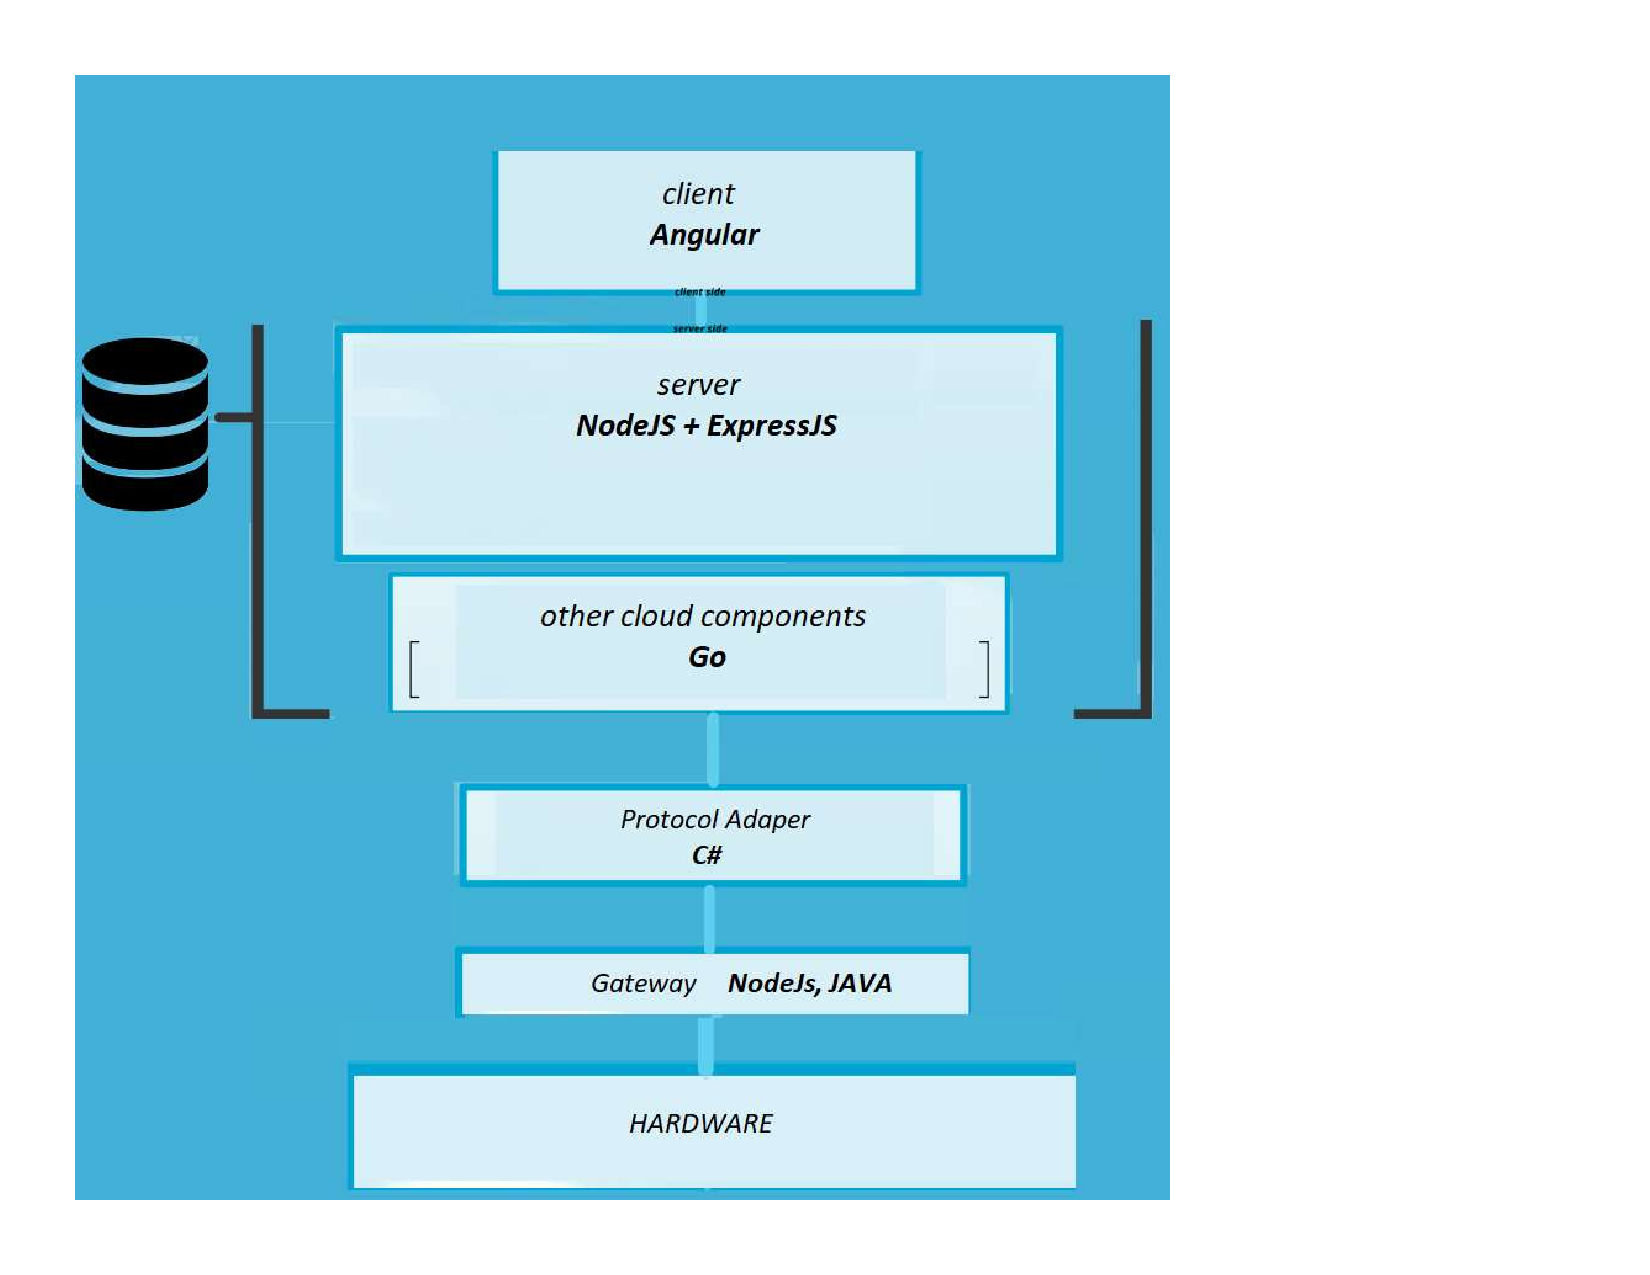
\includegraphics[width=0.70\textwidth,]{architecture.pdf}
	\caption{BOIC architecture}
	\label{fig:BOIC architecture}
\end{figure}

	\subsection{Description of the Continuous Deployment Environment }
	



% Ludwig: If these have been addressed, we can remove them.
%\todo{How did you reduce the number of values of these 2 Parameters !?! This is crucial!
%You applied some methodologies from Rachels paper - good, but which were those?, why did you choose exactly those?
%I propose a structure like this:
%\begin{itemize}
%	\item You describe the IPM for these two parameters before you modified them.
%	\item You describe which patterns (in rachles terms) you identified
%	\item ``This justifies to apply pattern X and/or pattern Y, to modify the parameter values.
%	... and we need to add this, and that constraint.''
%	\item So that the out coming IPM for these parameters looks like this: ....
%	\item This means we reduced the parameter sizes from 123 to 23 and 123 to 37 respectively (note these are dummy values).
%\end{itemize}
%}

		Refer to figure~\ref{fig:IBMmethodBlocks}. 
	Related parameter groups are henceforth referred to by color groups.
	In the figure the green path is described as when the Object Type is either analog input (AI), analog output (AO),
	analog value (AV), binary output (BO) or multisate output (MO). 
	When this is the case the related fields are enabled and the others are disabled.
  The teal path signifies another group of related parameters: binary input (BI), binary value (BV). 
	The blue path with multistate value (MV) works with the same logic.
	
		The 'enabling' of related parameters occurs as the parameter used for control of that parameter group is set to TRUE.
	Since only a single parameter group should be enabled at a time,
	through constraints, the other control parameters which control other groups are set to FALSE. 
	In turn, the parameter groups that are controlled by those control parameters are forced to have values equal to N/A.
	Here the use of N/A value for parameters that are not a part of the active parameter group in the current sequence 
	is an idea inspired from the modeling pattern referred to in section II C 1.
	The use of control parameters with values TRUE \& FALSE, 
	the use of the control logic to identify the sequence in which the parameter group is occurring 
	are ideas inspired from the modeling patterns referred to in section II C 3.
	

%	\begin{figure*}[!ht]
%	\centering
%		\includegraphics[width=1.00\textwidth]{IBMmethodIPMfullTable.pdf}
%	\caption{IPM of IBM method, full table}
%	\label{fig:IBMmethodIPMfullTable}
%	\end{figure*}
%

	A better way to represent this sequence logic would be to separate them in blocks.
	Figure~\ref{fig:IBMmethodBlocks} pictures how this can be structured.
	These blocks represent different UIs
	the user is presented with based on their parameter choices for the base block.
	The base block contains the parameters ObjectType and EventType,
	which are common to all paths. ObjectType's parameter values
	AI, AO, AV, BO, MO enable block 1 highlighted in green. ObjectType's parameter values BI
	and BV enable to block 2 highlighted in teal.
	ObjectType's last parameter value MV relates to block 3 highlighted in blue.
	
	Block 1 (in green) contains the parameters SetPointOrFeedbackPropType, SetPointOrFeedbackPropProperty.
	
	Block 2 (in teal) contains the parameters ObjectPropertyReferenceMV, PropertyStateType, ValueUnsigned.
	
	Block 3 (in blue) contains the parameters ObjectPropertyReferenceBVBI, PropertyStateType, ValueBinary.
	
	Notice PropertyStateType being common in both blocks. Depending on the choices in ObjectType
	of the base block, a default parameter value gets selected for PropertyStateType:
	binary when ObjectType is binary-input or binary-value, Unsigned when ObjectType is Unsigned.
	We will exemplify the 3 different sequences that may occur based on the initial choices of the user in the base block.
	
	Example 1: User selects ObjectType = 'AO', EventType = 'floating-limit' or 'out-of-range',
	the next set of configurations can only be for SetPointOrFeedbackPropType (over 2 choices under it)
	and SetPointOrFeedbackPropProperty (25 choices under it). 
	All other parameters set to N/A utilizing constraints. 
	
	Example 2: User selects ObjectType = 'MV', EventType = 'change-of-value',
	the next set of configurations can only be for ObjectPropertyReferenceMV (True or False),
	PropertyStateType (only Unsigned), ValueUnsigned (4 configurations). 
	All other parameters set to N/A utilizing constraints. 
	
	Example 3: User selects ObjectType = 'BV', EventType = 'change-of-state',
	the next set of configuration con only be for ObjectPropertyReferenceBVBI (True or False),
	PropertyStateType (only Binary), ValueBinary (00, 01, 10, 11).
	All other parameters set to N/A utilizing constraints. 

%	\begin{figure*}[!th]
%		\centering
%			\includegraphics[width=1.00\textwidth]{IBMmethodBlocks.pdf}
%		\caption{IBM method, blocks}
%		\label{fig:IBMmethodBlocks}
%	\end{figure*}
	
	A better understanding can be achieved by observing the verbal constraints.
	The Javascript code will be revealed in a later section while analyzing the pros and cons of the method. 
		
	\textsl{If ObjectType = AI,AO,AV  then  EventType = floating-limit	OR  out-of-range}
				
	\textsl{If ObjectType = BO,MO then EventType = command-failure	}			
	
	\textsl{If ObjectType = MV then EventType = change-of-value}
	
	\textsl{If ObjectType = AI,AO,AV,BO,MO then ObjectPropertyReferenceAIAOAVBOMO = TRUE
	ObjectPropertyReferenceMV = FALSE, ObjectPropertyReferenceBVBI = FALSE, PropertyStateType = N/A,
	ValueBinary = N/A, ValueUnsigned = N/A	}		
	

	\textsl{If ObjectType = BI,BV then EventType =change-of-state,  ObjectPropertyReferenceBVBI = TRUE,
	PropertyStateType = Binary, ObjectPropertyReferenceAIAOAVBOMO = FALSE, SetpointOrFeedbackPropType = N/A,
	SetpointOrFeedbackPropProperty = N/A, ObjectPropertyReferenceMV = FALSE,  ValueBinary != N/A, ValueUnsigned = N/A} 				
	

	\textsl{If ObjectType = MV then EventType = change-of-value, ObjectPropertyReferenceMV =  TRUE,
	PropertyStateType = Unsigned, ValueUnsigned != N/A, ObjectPropertyReferenceAIAOAVBOMO = FALSE,
	SetpointOrFeedbackPropType = N/A, SetpointOrFeedbackPropProperty = N/A, ObjectPropertyReferenceBVBI = FALSE,
	ValueBinary = N/A}

		
%	\subsection{Ideas to reduce parameter values}
%	In addition to equivalence-partitioning parameter values in block 1
%	(refer to block 1 example from the previous section) 
%	
%	While configuring for a MV (refer to block 2 example from the previous section) 
%	another idea came to mind. For the parameter ValueUnsigned, instead of many possible configurations, 
%	it appeared that a covering array can be utilized. 
%	Figure shows the UI for what configures the parameter named ValueUnsigned in the IPM: when the object of concern is an MV, 
%	the PropertyStateType is set to Unsigned and these are the values the user is presented with for the configuration.	

	
%	\begin{figure}[!h]
%		\includegraphics[width=0.50\textwidth]{subCoveringArray.pdf}
%		\caption{configuring parameter values in the UI}
%		\label{fig:subCoveringArray}
%	\end{figure}
%	
%	Evaluating the configurations in a table, it was realized that there are in fact 8 possible ways to configure the value. The states that lead to the configurations are detailed in Figure~\ref{fig:subCoveringArrayTable}. In a sub-IPM, the states were then taken as parameters themselves, their True/False states as parameter values and plugged in NIST's Automated Combinatorial Testing for Software tool (ACTS) \cite{o2009automated} .  The resulting covering array showing the 4 configurations (Config6, 5, 3, 0) can be observed in Figure~\ref{fig:subCoveringArrayTable}.
%	
%	\begin{figure}[!h]
%		\centering
%			\includegraphics[width=.50\textwidth]{subCoveringArrayTable.pdf}
%		\caption{8 possible configurations in UI, reduced to a covering array}
%		\label{fig:subCoveringArrayTable}
%	\end{figure}
	

%	\subsection{Modeling BACnet with SBA-Method}
%	In \cite{kampel2017combinatorial} a combinatorial methodology to model composed software systems is presented.
%	The main idea behind this methodology is to combine legacy test suites of the components,
%	via a so called \emph{meta-array}, to get a test suite for the whole SUT.
%	It is also shown that, if the legacy test suites, as well as the meta-array fulfill certain combinatorial creteria,
%	so does the test suite for the whole SUT (for details see \cite{kampel2017combinatorial}.)
%	
%	
%	The SBA-Method \cite{kampel2017combinatorial}, can be summarized in 5 core steps. Each step will be detailed in subsequently.
%	
%	\subsubsection{ Generate seed covering array (CA) for strength t=1 for each of the parameter partitions} 
%	We start by dividing the interrelated parameter groups into seeds.
%	 \todo{Ludwig, please insert a short description of what seeds are, perhaps make a reference to a paper, maybe this one? \cite{kampel2017combinatorial}  } 
%	In identifying the seeds for an EEO, we borrow initial ideas from the IBM method for separating the sequenced parameter groups. 
%	The parameters and values that make possible the IBM method; parameters that enable/disable blocks (using TRUE and FALSE), parameter values that are 'N/A' which disable blocks, are not needed.
%	Refer to the IPM in Figure~\ref{fig:IBMmethodIPMfullTable}. 
%	The second important point is that each seed gets its unique parameters whether they are common in the other seeds or not: in the figure these are ObjectType and EventType parameters which are common in the seeds but their parameter values are different based on user selection. 
%	For example in seed2: if ObjectType is BI or BO, EventType is set to changeOfState immediately and the ValueBinary can have values from 00 to 11. 
%	Another example is in seed3: if ObjectType is MV, EventType is set to changeOfValue and ValueUnsigned is one of the 8 configurations, of which we are using 4 as described in Figure~\ref{fig:subCoveringArrayTable}. 
%	Once the seeds are defined, we start generating a CA for strength t=1. In Figure~\ref{fig:Step2} 1-way covering arrays are shown in ACTS screenshots: seed1 has 37 tests, seed2 and seed 3 have 4 tests each.
	
	
%	\begin{figure}[h]
%		\centering
%			\includegraphics[width=.50\textwidth]{step1.pdf}
%		\caption{SBA method Step 1}
%		\label{fig:step1}
%	\end{figure}
	
	
% \subsubsection {Generate a meta CA of strength t=2; the input is an IPM where each parameter corresponds to a partition and the parameter values are integers from 1 to the size of the respective seed CA (from step 1) } Here seed1 corresponds to partition M1, seed 2 to M2 and so on. Each test in the seed is represented by an integer: 37 in M1, 4 in M2 and 4 in M3. Following this a meta CA is generated of strength 2 (t=2 : 2-way). The meta array in our example has 148 tests as shown in the ACTS screen shot in Figure~\ref{fig:Step2}
	
		
%	\begin{figure}[!h]
%		\centering
%			\includegraphics[width=0.50\textwidth]{Step2.pdf}
%		\caption{SBA method Step 2}
%		\label{fig:Step2}
%	\end{figure}
	
	
%	\subsubsection {Expand step 1 and 2 with real values instead of numbers: apply the plug-in construction: } In this step we take our meta array with 148 tests and expand it with real values. In Figure~\ref{fig:step3} shows the entirety of parameters:  
%	M1: ObjectType, EventType, SetPointOrFeedbackPropType, SetPointOrFeedbackPropProperty; 
%	M2: ObjectType, EventType, ValueBinary; 
%	M3:ObjectType, EventType, ValueUnsigned .
%	Parameter M1 has 37 possible values used in 148 tests (refer to step 1 and 2), so the integers 1 to 317 get replaced with the tests in step1. 
%	Parameter M2 has 4 possible values in 148 tests, so the integers 1 to 4 get replaced with the tests in step1 and so on for M3.
		
	
%	\begin{figure}[!h]
%		\centering
%			\includegraphics[width=0.50\textwidth]{step3.pdf}
%		\caption{SBA method Step 3}
%		\label{fig:step3}
%	\end{figure}
	
	
%	\subsubsection {Generate juxtaposed CAs of strength 2 for each of the partitions: } Refer back to step1 where we created seed CAs for strength t=1 (seed out) as shown in Figure~\ref{fig:Step2}. 
%	In this step we have a parallel effort where we create the same CAs with strength t=2 (jux out: juxtaposed out) instead. 
%	In Figure~\ref{fig:step4 and 5} these 2-way CAs can be observed: 925 2-way tests for seed1, 8 2-way tests for seed2 and 4 2-way tests for seed3. 
	
%	\begin{figure}[!h]
%		\centering
%			\includegraphics[width=0.50\textwidth]{step4&5.pdf}
%		\caption{SBA method Steps 4 and 5}
%		\label{fig:step4 and 5}
%	\end{figure}

\subsection{Description of the Test Code Structure}
	
All t-way coverage measurements were made using NIST's coverage measurement tool Combinatorial Coverage Measurement (CCM) command line version \cite{kuhn2013combinatorial}.

	For IBM method, the coverage with constraints factored in and the coverage without constraints are examined in figures~\ref{fig:coverageIBM-UH} and~\ref{fig:coverageIBM-UH_noConstraints}.
Figure~\ref{fig:coverageIBM-UH} shows the 2, 3, 4-way coverage measurement of the IBM method, respectively figure~\ref{fig:coverageIBM-UH_noConstraints} shows the coverage measurement without constraints. 

%	\begin{figure}[h]
%		\centering
%			\includegraphics[width=0.50\textwidth]{coverageIBM-UH.pdf}
%		\caption{Coverage: IBM method}
%		\label{fig:coverageIBM-UH}
%	\end{figure}
%	
%	\begin{figure}[h]
%		\centering
%			\includegraphics[width=0.50\textwidth]{coverageIBM-UH_noConstraints.pdf}
%		\caption{Coverage: IBM method without constraints}
%		\label{fig:coverageIBM-UH_noConstraints}
%	\end{figure}

As mentioned in Section III B, the use of constraints are at the foundation of the IBM method. 
The 2-way coverage without constraints is at 100\% as seen in figure~\ref{fig:coverageIBM-UH_noConstraints}.
The application of constraints, which make the method possible, reduces the 2-way coverage measurement to 58.1\%. Because constraints are an integral part of the method, in this evaluation we believe that the coverage measurement of the IBM method is inconsequential. 

For SBA method, the coverage with constraints factored in and the coverage without constraints are examined in figures~\ref{fig:coverageSBA} and~\ref{fig:coverageSBA_noConstraints}.
Figure~\ref{fig:coverageSBA} shows the 2, 3, 4-way coverage measurement of the SBA method, respectively figure~\ref{fig:coverageSBA_noConstraints} shows the coverage measurement without constraints.
The 2-way coverage without constraints is at 100\% as seen in figure~\ref{fig:coverageSBA_noConstraints}. The minimum 2-way coverage without constraints is also at 100\%. 

The significance and the impact of minimum t-way coverage on branch coverage conditions in the code is discussed in paper \cite{kuhn2016measuring}. 
Label M as the minimum 2-way coverage; i.e., the lowest proportion of settings covered for all t-way combinations of variables. 
For example, 2-way combinations of binary variables have four possible settings: 00, 01, 10, 11. Some variable pairs may have all four settings covered, but others may have less. 
M is the smallest proportion of coverage among all of the t-way variable combinations.  M is also viewable as the rightmost line in the coverage strength meters in Figure 1 and 3. 

%\begin{figure}[h]
%	\centering
%		\includegraphics[width=0.50\textwidth]{coverageSBA.pdf}
%	\caption{Coverage: SBA method}
%	\label{fig:coverageSBA}
%\end{figure}
%
%	\begin{figure}[h]
%	\centering
%		\includegraphics[width=0.50\textwidth]{coverageSBA_noConstraints.pdf}
%	\caption{Coverage: SBA method without constraints}
%	\label{fig:coverageSBA_noConstraints}
%\end{figure}

Applying the constraints to the SBA method has a miniscule impact on the overall 2-way coverage: down from 100\% to 99.76\% as seen in figure~\ref{fig:coverageSBA}. 
The effect on 3 and 4-way coverage is similar. 
\todo{Ludwig, do you want to insert a sentence on why this is?}
The impact of constraints on the minimum 3-way and 4-way coverage is non-existent, however on minimum 2-way coverage the difference is 40\%. \todo{Ludwig, do you want to insert a sentence on why this is?}.
Overall, t-way coverage analysis is valid on the SBA method. 
	
	\subsubsection {Vertically juxtapose the juxtaposed CAs in step 4 to the result of step 3. This guarantees that the final result is again a 2-way covering array: } We simply add the 2-way CA under the 1-way CA as shown in Figure~\ref{fig:step4 and 5}. Here the first seed has 925 tests while the others have 8 and 4 respectively, this may seem challenging at first. 
	For seed 2 and 3 we simply, repeatedly keep adding in blocks (of 8 and 4 respectively) until we cannot add anymore. If the final addition is not a multiple of 925, then we add the remainders. 

\section{Test Methodology}
	
	In the following sections the coverage measurements, the pro's and con's of the IBM and the SBA methods will be evaluated. 
		
	
	\subsection{Input driven testing of hardware}
	
	Considering t-way coverage measurement, SBA method provides evidence of the measurement while coverage measurement in IBM method is inconsequential as explained in the previous section. 
		
	Regarding the Application of the methods, IBM method is straightforward once the constraints are figured out. 
	SBA method has elaborate steps as outlined in section III D. 
	In step 3 of the method (plug-in construction), there is a need for a script that replaces integers with real values.
	Currently a freely available tool does not exist for such a task.
	
	Constraints are important for both methods, but they are vital for IBM method. 
	They can be manageable in a small scale, yet as the SUT gets larger they get more complicated. 
	Figure~\ref{fig:constraintsIBM-UH} shows the Javascipt code for constraints used in the IBM method.
	
% can we put this picture on the same page as the section?	
%\begin{figure*}[!bth]
%	\centering
%		\includegraphics[width=.90\textwidth]{constraintsIBM-UH.pdf}
%	\caption{Constraints in JavaScript, IBM method}
%	\label{fig:constraintsIBM-UH}
%\end{figure*}

	Considering the above factors, IBM method may be preferred for smaller systems under test while SBA method may be preferred for larger systems.
	However, the significance of the above factors for the system and/or the test team may effect the preferences for the method of use.

	\subsection{Filtering Points by Tag Combinations }

	\subsection{State Transitions Between Combinations of Alarm Data, With a Variable Oracle}

	\subsection{Sequenced Filtering, Searching, Sorting of Geo-located Sites}
	
\section{Conclusion and future work}
	
The initial challenge in this study was how to best test EEO configurations in the most efficient manner.
During the study it became apparent that the methods applied can be used to test any system where the parameter groups for
the Combinatorial Input Parameter Model (IPM) are not simultaneously available, and instead may appear sequentially.
Future work on this front may incorporate system test ideas where each seed (in the SBA method) or different color (in the IBM method) being a different module of functionality.

\textbf{Acknowledgments.}
This research was carried out in the context of Austrian COMET K1
program and publicly funded by the Austrian Research Promotion Agency
(FFG) and the Vienna Business Agency (WAW).

\bibliographystyle{IEEEtran}
\bibliography{cloud}

\end{document}
